\documentclass[tikz,convert={outfile=\jobname.svg}]{standalone}
%\usetikzlibrary{...}% tikz package already loaded by 'tikz' option
\begin{document}
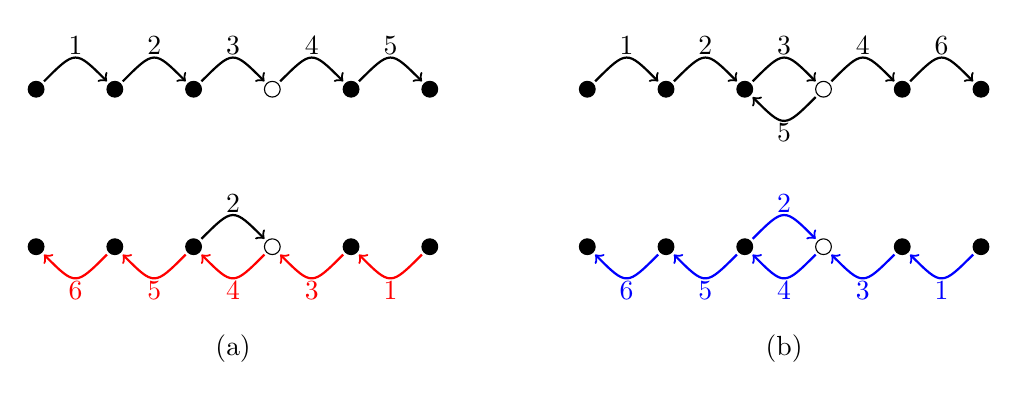
\begin{tikzpicture}
    \def\dx{0}
    \foreach \x in {1,...,5}
        \draw [->,thick] (\x+\dx-0.9,0.1) .. controls (\x+\dx-0.5,0.5) .. (\x+\dx-0.1,0.1)
        node[pos=0.5,yshift=1ex]{\x};
    \foreach \x in {3}
        \filldraw[fill=white] (\x+\dx,0) circle [radius=0.1];
    \foreach \x in {0,1,2,4,5}
        \filldraw[fill=black] (\x+\dx,0) circle [radius=0.1];
    % bottom
    \def\y{-2.0};
    \foreach[evaluate={\j=\x==1?\x:int(\x+1)}] \x in {5,...,1}
        \draw [red,<-,thick] (5.1-\x+\dx,\y-0.1) .. controls (5.5-\x+\dx,\y-0.5) .. (5.9-\x+\dx,\y-0.1)
        node[pos=0.5,yshift=-1ex]{\j};
    \foreach \x in {2}
        \draw [->,thick] (\x+\dx+0.1,\y+0.1) .. controls (\x+\dx+0.5,\y+0.5) .. (\x+\dx+0.9,\y+0.1)
        node[pos=0.5,yshift=1ex]{\x};
    \foreach \x in {3}
        \filldraw[fill=white] (\x+\dx,\y) circle [radius=0.1];
    \foreach \x in {0,1,2,4,5}
        \filldraw[fill=black] (\x+\dx,\y) circle [radius=0.1];
    \draw (2.5,-3.3) node {(a)};

    % reversible computing
    \def\dx{7}
    \foreach[evaluate={\j=\x==5?int(\x+1):\x}] \x in {1,...,5}
        \draw [->,thick] (\x-0.9+\dx,0.1) .. controls (\x-0.5+\dx,0.5) .. (\x-0.1+\dx,0.1)
        node[pos=0.5,yshift=1ex]{\j};
    \foreach \x in {3}
        \draw [<-,thick] (\x-0.9+\dx,-0.1) .. controls (\x-0.5+\dx,-0.5) .. (\x-0.1+\dx,-0.1)
        node[pos=0.5,yshift=-1ex]{5};
    \foreach \x in {3}
        \filldraw[fill=white] (\x+\dx,0) circle [radius=0.1];
    \foreach \x in {0,1,2,4,5}
        \filldraw[fill=black] (\x+\dx,0) circle [radius=0.1];
    % bottom
    \def\y{-2.0};
    \foreach[evaluate={\j=\x==5?int(6-\x):int(7-\x)}] \x in {1,...,5}
        \draw [blue,<-,thick] (\x-0.9+\dx,\y-0.1) .. controls (\x-0.5+\dx,\y-0.5) .. (\x-0.1+\dx,\y-0.1)
        node[pos=0.5,yshift=-1ex]{\j};
    \foreach \x in {2}
        \draw [blue,->,thick] (\x+0.1+\dx,\y+0.1) .. controls (\x+\dx+0.5,\y+0.5) .. (\x+\dx+0.9,\y+0.1)
        node[pos=0.5,yshift=1ex]{\x};
    \foreach \x in {3}
        \filldraw[fill=white] (\x+\dx,\y) circle [radius=0.1];
    \foreach \x in {0,1,2,4,5}
        \filldraw[fill=black] (\x+\dx,\y) circle [radius=0.1];
    \draw (2.5+\dx,-3.3) node {(b)};
\end{tikzpicture}
\end{document}
